%% LaTeX template for BSc Computing for Games final year project dissertations
%% by Edward Powley
%% Games Academy, Falmouth University, UK

%% Based on:
%% bare_jrnl.tex
%% V1.4b
%% 2015/08/26
%% by Michael Shell
%% see http://www.michaelshell.org/
%% for current contact information.
%%
%% This is a skeleton file demonstrating the use of IEEEtran.cls
%% (requires IEEEtran.cls version 1.8b or later) with an IEEE
%% journal paper.
%%
%% Support sites:
%% http://www.michaelshell.org/tex/ieeetran/
%% http://www.ctan.org/pkg/ieeetran
%% and
%% http://www.ieee.org/

%%*************************************************************************
%% Legal Notice:
%% This code is offered as-is without any warranty either expressed or
%% implied; without even the implied warranty of MERCHANTABILITY or
%% FITNESS FOR A PARTICULAR PURPOSE! 
%% User assumes all risk.
%% In no event shall the IEEE or any contributor to this code be liable for
%% any damages or losses, including, but not limited to, incidental,
%% consequential, or any other damages, resulting from the use or misuse
%% of any information contained here.
%%
%% All comments are the opinions of their respective authors and are not
%% necessarily endorsed by the IEEE.
%%
%% This work is distributed under the LaTeX Project Public License (LPPL)
%% ( http://www.latex-project.org/ ) version 1.3, and may be freely used,
%% distributed and modified. A copy of the LPPL, version 1.3, is included
%% in the base LaTeX documentation of all distributions of LaTeX released
%% 2003/12/01 or later.
%% Retain all contribution notices and credits.
%% ** Modified files should be clearly indicated as such, including  **
%% ** renaming them and changing author support contact information. **
%%*************************************************************************


\documentclass[journal]{IEEEtran}

\usepackage{graphicx}
% Insert additional usepackage commands here
\usepackage[hyphens]{url}
\usepackage[hidelinks]{hyperref}

\begin{document}
%
% paper title
% Titles are generally capitalized except for words such as a, an, and, as,
% at, but, by, for, in, nor, of, on, or, the, to and up, which are usually
% not capitalized unless they are the first or last word of the title.
% Linebreaks \\ can be used within to get better formatting as desired.
% Do not put math or special symbols in the title.
\title{Barriers preventing elderly in care home playing video games and potential ways around this}
%
%
% author name
\author{Steven Cowie - 1605240 }

% The paper headers -- please do not change these, but uncomment one of them as appropriate
% Uncomment this one for COMP320
\markboth{COMP320: Research Review and Proposal}{COMP320: Research Review and Proposal}
% Uncomment this one for COMP360
% \markboth{COMP360: Dissertation}{COMP360: Dissertation}

% make the title area
\maketitle

% As a general rule, do not put math, special symbols or citations
% in the abstract or keywords.
\begin{abstract}
This paper examines how the use of a new design methodology could be used to help elderly citizens in care home play video games, without the struggles they might normally find if they tried to play a regular game. It also looks into the problems they face and ways to overcome this. A new controller will be designed to play the games they are most interest in and it will be evaluated to see how well it works. An interface will also be part of the game with a set of guidelines that will be followed to make the game as user friendly as possible to the elderly. As games have so many benefits and being so enjoyable it is only right that as many people can play them.
\end{abstract}

\section{Introduction}
% The very first letter is a 2 line initial drop letter followed
% by the rest of the first word in caps.
% 
% form to use if the first word consists of a single letter:
% \IEEEPARstart{A}{demo} file is ....
% 
% form to use if you need the single drop letter followed by
% normal text (unknown if ever used by the IEEE):
% \IEEEPARstart{A}{}demo file is ....
% 
% Some journals put the first two words in caps:
% \IEEEPARstart{T}{his demo} file is ....
% 
% Here we have the typical use of a "T" for an initial drop letter
% and "HIS" in caps to complete the first word.
\IEEEPARstart{T}{his} project aims to look into two issues. The first, being the common challenges the elderly in care home face while they want to play video games. The second is how can a new standard design methodology be created to make games more accessible to the elderly and then it will be evaluated. This will feature an interface and a new controller to try and overcome these issues to to allow more elderly users in care home to play and enjoy games. 
\newline
This paper will take into account the majority of the issues that the elderly have trouble with when it comes to playing video games and attempt to condense them down into a standard design methodology for future developers. It will focus on the games the elderly in particular like to play so it is more directly aimed at the whole user base. If it was done for every type of game it would be too difficult as the elderly prefer certain game types \cite{whitcomb_computer_1990} and do not like the others as they aren't into the same types of games \cite{whitcomb_computer_1990}.
\newline 
It is estimated that in the UK that by 2030 there will be fifteen and a half million  residents over the age of 65 \cite{noauthor_ageing_nodate}. With that being said the elderly offer a very large potential customer base \cite{ijsselsteijn_digital_2007}. This market is widely unexplored in terms of games and therefore if explored further this could lead to a niche market being created and potentially expanded into a more broad market for the elderly. The BBC did some research and found that people over that age of 65 were the most likely age group to be watching TV and their favorite activity is TV but they are the least likely to be on a computer unless then need to be \cite{ijsselsteijn_digital_2007}. Games should be accessible to everyone but unfortunately that is not the case. Many users suffers from disabilities or they have needs which makes it too difficult for them to play what everyone else plays \cite{torrente_introducing_2011}. For everyone to experience gaming in the same way and get all the benefits out of it is based on their experience based on the impairments they have \cite{gerling_long-term_2015}.

\subsection{Benefits of Video Games for the Elderly}
When being played everyone and especially by the elderly, video games have been proven to have several benefits to them which can help elderly people live a better life \cite{noauthor_video_nodate}. In today's society video games are also now being used for rehabilitation for several diseases and illness's \cite{hansen_robot_2011} \cite{gerling_long-term_2015}. The first benefit that can brought on through the use of video games is increased speed in your reaction time \cite{whitcomb_computer_1990} \cite{ijsselsteijn_digital_2007}, a study done showed that elderly users who played Pac Man and Donkey Kong reaction time sped up \cite{whitcomb_computer_1990}, this has been shown to help the elderly in other aspects of their lives such as driving ability \cite{whitcomb_computer_1990}. Other benefits were found during a study where twenty-one adults played games and found out there were therapeutic benefits which made them feel a sense of success and achievement as well as they made better constructive use of their leisure time \cite{whitcomb_computer_1990}, this could lead to an overall happier life. To further back the point up another study was looked at where they looked at elders who played games for five hours a week and found it improved their self esteem \cite{ijsselsteijn_digital_2007}. Contrary to belief the research aimed at elders in still in an early stage and opposite findings have been reported \cite{ijsselsteijn_digital_2007}, this can open the field to more research in this specific area.


\section{Usability and Accessibility}
There are two main factors when it comes to making games more  care home friendly for the elderly, they are usability and accessibility. 
\subsubsection{Accessibility} Accessibility determines how easily the users can play the game by using physical devices such as controllers \cite{hersh_accessibility_2012}, for example if you are a "normal" person with no physical disabilities or chronic pains you should have no trouble using any modern standard controller, but a disabled person on the other hand probably would struggle due to them having different needs to be able to use it. 
\subsubsection{Usability} Usability is how well the system delivers it's intended function with ease \cite{hersh_accessibility_2012}, for example most on screen interfaces are usable for the majority of users with no vision impairments, but then you have the elderly who commonly lose parts of their vision \cite{correia_global_2016} might struggle to read it so making it bigger for example would be better.

\section{Related Literature}
e-Adventure is a tool for used for creating educational games \cite{torrente_introducing_2011}. it is limited to being able to make point and click games only. It suggests being able to give users settings they can change based upon their needs and offers different levels depending on how bad someone's disability is, as well as suggesting for it to allow different variations of inputs, this allows the game to be configurable to wider audiences. Trying to find a good balance between the two is the key to trying to improve all round accessibility. 
\newline
Educational games is an area  where lots of research has been done as games are becoming more accepted for educational use too \cite{torrente_eyes-free_2012}, users are trying to make educational games for people with disabilities and that can link to the elderly through both of them can face some of the same issues. The paper Eyes-free Interfaces for Education Games \cite{torrente_eyes-free_2012} discusses what the player experience should be like, it says that the developers should ship games with configurable interfaces, this is commonly mentioned among papers. Next it recommends that the games should need to get more challenging as you go and that every user should be able to have a good experience playing the game but it has to try and feel the same for every player, if this isn't done correctly the player who may be struggling could feel let down and not want to continue playing.
\newline
Quite a lot of studies have been done into making controllers for the disabled, one in particular by Hawsawi and Sernwal \cite{hawsawi_eeg_2014} talks about the use of a headset as a controller for mobility impaired gamers. The EEG headset is designed for those users who have mobility impairments so it uses "brain activity, facial muscles and eye movement" as forms of input \cite{hawsawi_eeg_2014}. This could be a good solution but it only really caters to those who have mobility impairments and the normal user may find it uncomfortable. Video games are becoming very popular and the approximately eleven percent of the US population find it hard to play due to a disability \cite{hawsawi_eeg_2014}. Of the disabled gamers, two percent are unable to play at all and nine percent don't get the full experience \cite{hawsawi_eeg_2014}. Analysts say that accessibility is a low propriety for game developers but believe if they tried to make their games more accessible it could be huge \cite{hawsawi_eeg_2014}. They then go on to say that all the motor impairments cannot be addressed in cohesive whole so they look into users with cerebral palsy.

\section{Barriers Preventing Elderly Playing Video Games}
\subsection{Attitude}
One of the smallest barriers that are preventing elderly playing video games are themselves \cite{whitcomb_computer_1990}. They're not as open as younger generations when it comes to learning how and using new technology, a large percentage of them like sticking to what they know. Figures show that only nineteen percent of over 65's in the USA have a computer \cite{whitcomb_computer_1990}, this number is so small considering more and more things are moving online. A study done showed that 25 percent of 28 elders in a care home wanted to use a computer but after playing 2 separate games this figure rose up to 65 percent \cite{whitcomb_computer_1990}, this shows that allowing yourself to be open to new ideas, you might actually like it. The elder's lack of experience on computers is related to why they may dislike learning to play games \cite{gerling_exergame_2010}.
\newline
\newline
On another note it isn't just the attitude of the elders it's that of game developers too \cite{torrente_introducing_2011}, they may be unaware of people with disabilities needs and the costs associated with trying to find a way around this \cite{torrente_eyes-free_2012}. The cost associated for making up expensive interfaces for such a tiny percentage of their market isn't worth it \cite{torrente_eyes-free_2012}, which is one of the reasons doing this research could be beneficial to many users who want to play. Game developers have not taken advantage of the fact no one really makes games for the elderly which leaves potential for a niche in the market which could be huge money-wise if done correctly \cite{ijsselsteijn_digital_2007}.
\newline
From research that was done, they found out elderly citizens seemed to approve of the Nintendo Wii \cite{gerling_exergame_2010}, but at the same time most wii games using the balance board were designed for younger users and so only a few mini games were actually accessible for the elderly but these games can be used to improve their balance \cite{gerling_exergame_2010}, this is good because they still see a benefit.
\newline
Some elderly users may find it uncomfortable to play games in social situations if they are experiencing "vulnerability over their age-related changes and impairments." \cite{gerling_long-term_2015}, they may not want to show off their vulnerabilities, to potentially fix this they might find using an easier interface might make the game not as hard to play which might help. 


\subsection{Modern Games}
The elderly aren't into the same sorts of games as younger people who game \cite{ijsselsteijn_digital_2007}. This is due to them seeking a more rewarding experience instead of caring about performance in the game \cite{ijsselsteijn_digital_2007}, hence why when a study was done it found that hangman and trivia games were their favorite to play  from certain options \cite{whitcomb_computer_1990}. They do not like how vulgar some games are \cite{whitcomb_computer_1990}. As well as that they couldn't keep up with what was going on due to some games being too fast, or objects were too small for them to make out clearly what they were \cite{whitcomb_computer_1990}, to overcome this issue every game should have usability settings that allow the user to customize the UI. Small objects moving too quickly though is commonly seen in action games.
\subsubsection{Games the elderly like}
These days it seems like the elderly do play more games than before, however most of these games seem to be on a digital tablet \cite{jenkin_rise_2014}. From research it is clear that the elderly prefer simple games, games that could be play without the need for a digital interface, the best examples of these are cards games and puzzle/trivia games \cite{noauthor_nearly_nodate}, to back this out Whitcomb found out when he did his study that their favorite games were trivia and hangman \cite{whitcomb_computer_1990}. These could also be their favorite types of games because they are simple enough to play. 

\subsection{Usability}
Usability is where lots of game developers fall down, a few simple additions to their settings menus could make the game accessible for so many more users. EA have been one of the few companies to do this and they've even launched an accessibility forum \cite{noauthor_ea_nodate}. A few simple features they've added are giving the player the option to enlarge clickable targets, remap buttons and sticks on the actual controller and a pause menu that only lets the user use a mouse \cite{mcaloon_look_nodate}.
\newline
Games accessibility guidelines \cite{noauthor_game_nodate} is a website which provides three separate lists; basic, intermediate and advanced which break down into categories. The categories are motor, cognitive, vision, hearing, speech and general. It lists features, depending on the level you select, that games should have, this list proves to be very useful for developers and more of them should look at it, a few things listed by them will be used to help with the design methodology for the elderly. 

\subsubsection{Vision Impairments}
As the elderly grow older they can naturally develop loss of sight \cite{loh_age_2004} \cite{ijsselsteijn_digital_2007}. This can cause them to have glare problems \cite{ijsselsteijn_digital_2007} which can make it difficult to see whats on the interface if it's too small, for example captions of objectives on screen. Digital Game Design for the Elderly Users \cite{ijsselsteijn_digital_2007} suggest that you should give the user control over the font, colour, contrast settings, window resizing, scroll rate and zooming \cite{ijsselsteijn_digital_2007} , this would help to make it better for those who struggle to see as it allows it to be more suited towards the users needs. Games accessibility guidelines \cite{noauthor_game_nodate} says that a colour alone should not be the only way a user can be told essential information, which is why tactile feedback would be good \cite{ijsselsteijn_digital_2007}.

\subsubsection{Cognitive Impairments}
The games accessibility guideline suggests that games shouldn't have lots of menus before the user can play, some users might struggle especially if they have short term memory loss \cite{noauthor_game_nodate}.

\subsubsection{Hearing Impairments}
Elderly people develop loss of sound at certain frequencies \cite{ijsselsteijn_digital_2007} and for this reason if games feature high pitch noises they might not hear them. To counter against this issue tactile feedback is suggested \cite{ijsselsteijn_digital_2007} so the user still has the same experience. Subtitles should also be able to be used to make it easier if they are hard of hearing \cite{noauthor_game_nodate}.

\subsection{Accessibility}
It has been predicted that the number of carers for those with disabilities and the elderly will decrease but the amount of elders and disabled people will rise \cite{hansen_robot_2011}, this is bad news for care homes as it means less staff per person, which leads to less attention per person. 
\subsubsection{Arthritis}
One of the biggest issues that can make it difficult for the elderly to use a controller is their grip strength if they have arthritis \cite{noauthor_managing_nodate}, due to the fact it weakens their grip strength, there are however exercises that can be done to try and fix these \cite{noauthor_managing_nodate}. A study was done that showed a potential linking that games controllers and the use of mobile phones may even cause arthritis \cite{noauthor_games_2011} so for an elderly user who may already be suffering from this, this is the last thing they'd want. 
\newline
\begin{figure}[!h]
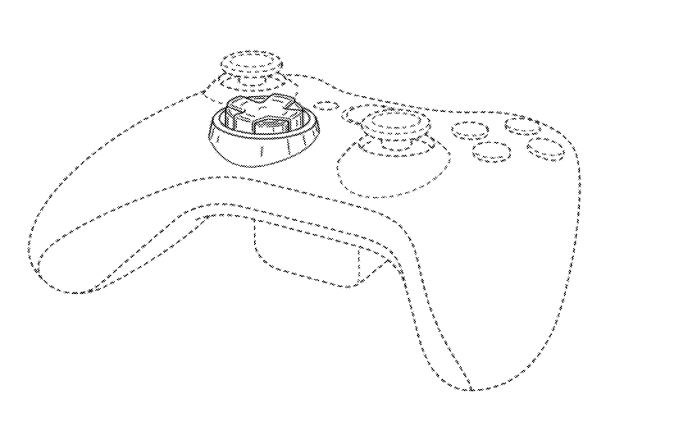
\includegraphics[width=0.5\textwidth]{controller.JPG}
\caption{Xbox 360 Controller \cite{ikeda_game_2012} }
\label{fig:primingweb-img}
\end{figure} \textbf{Fig 1} Image showcasing what most controllers these days look like. 
\newline
Figure 1 is what your typical controller looks like, this one being the patent for the Xbox 360. With the natural aging process you have a high chance of developing arthritis which is why an estimated nine million people affected by it in the UK alone \cite{noauthor_arthritis_2017}. The problem there being it makes it very difficult to hold a controller at all for some users \cite{gamecentral_perils_2016}, never mind for long periods of time. If users struggle to even pick up the controller then that essentially puts joysticks out of the question because they need their hand to be able to move freely. Unfortunately this is what most modern controllers are like these days.

\subsubsection{Motor Impairments}
Based on the condition of the users motor impairments it can lead to "slower response times, decline in the ability to maintain continuous movements, disruptions in coordination and balance, loss of flex ability, and greater variability in movement" \cite{ijsselsteijn_digital_2007}. This means games with fast reaction times are not good for them if they have slower response times due to the them having slower hand-eye coordination and don't have the ability to process things as fast \cite{ijsselsteijn_digital_2007}. A study done showed that using push buttons only were good for users who had cerebral palsy \cite{soto_online_2015}, this could be a good idea as there is no need for precise analogue stick movement. Also in Digital Game Design for Elderly Users backs up the point saying controllers should be buttons only by mentioning that elderly users can struggle to steady the mouse for accurate movements \cite{ijsselsteijn_digital_2007}.

\subsubsection{Controller Ergonomics}
The Ergonomic Development of Video Game Controllers \cite{bhardwaj_ergonomic_2017} talks about modern day controllers and how they are build to fit to most users. It then discusses button sizes on controllers and how there is an ideal diameter of 13-25mm to fit most users, so for elderly users they would probably prefer buttons on the larger size of that scale or even bigger. As well as button size it mentions that the force needed to push on these buttons should be less than 5.6N which all of the controllers they tested fall into, this just makes it easier if the elderly have problems with grip \cite{noauthor_managing_nodate}.

\subsubsection{Staff}
The staff in a care home are the perfect people to help users who have certain needs be able to play games or to just make them more comfortable playing games \cite{gerling_long-term_2015}, this could lead to more games being played by the elderly in care homes.

\section{Solutions}
\subsection{Alternative Controllers}
A potential solution to make it easier for the elderly to play video games is to seek the use of an adapted controller or attachments for the standard controller, this helps improve accessibility \cite{noauthor_xbox_nodate-1}.
\subsubsection{Xbox Adaptive Controller}
The Xbox adaptive controller \cite{noauthor_xbox_2018} is the first large commercially available controller that is designed for disabled users, but the elderly could make good use of it if it was adapted for them. It is essentially two large buttons with a small D-pad but has many expansions slots on the back allowing for maximum customization, for example you are able to purchase many forms to mount the controller as well as a range of buttons to suit your needs \cite{noauthor_xbox_nodate}.

\subsubsection{Avenger Controller}
An article done on Gunnar.com \cite{noauthor_ergonomics_2012} discusses the Avenger Adapter \cite{noauthor_avenger_nodate} for modern controllers. It is a device which wasn't designed for ergonomics \cite{noauthor_ergonomics_2012} but to give you an advantage while playing games \cite{noauthor_avenger_nodate}. It snaps onto the controller and allows the user to make it so that they don't need to use the buttons on the right hand side anymore since they have plastic toggles going over the back and side. This allows the user to be able to readjust the position of where they want them to be as well as the response time by tightening them up. The person who reviewed this claims it helped with cramps \cite{noauthor_avenger_nodate}.

\subsubsection{Tablet}
With more and more tablets being available these days at lower price points the elderly users could make use of tablets for gaming as well as their other computing needs \cite{noauthor_safest_2014}. The iPad is good for the elderly as it comes with a wide range of accessibility features which makes it easy to use for people with all sorts of needs \cite{noauthor_accessibility_nodate}. With Apples simple iOS \cite{noauthor_3_nodate} it makes it easier for users of all ages to navigate. With tablets being so easy to use, there are such a wide array of applications that are available and there if we are going off that the elderly like to play card games and puzzle and trivia games \cite{noauthor_nearly_nodate}) then app stores such as Apples own one \cite{noauthor_app_nodate} have plenty in store for them.

\section{Method}
The aim of this project is whether a new design methodology of a controller to go with it an interface makes the games more accessible for the elderly in care homes and to test it out I will be using a system usability score with the help of a questionnaire to get feedback from participants to evaluate how well the design works.
\subsection{Tools}
Three main tools will be used to conduct the methodology, they are Unreal Engine 4, Arudino and Arduino IDE.
\subsubsection{Unreal Engine 4}
The first being Unreal Engine 4 \cite{noauthor_what_nodate}. Unreal Engine 4 is one of the 2 most frequently used games engines, triple A studios use it make titles such as Fortnite \cite{noauthor_fortnite_2018} which won game of the year at the Joystick Awards \cite{noauthor_fortnite_2018-1}, so this will provide more than enough power for what is planned on being made. This will be used to allow me to design and program the game that will be made which will be used in testing. It is good because it gives you lots of control as to what you want it to do and it can easily allow you to program tools for usability. 
\subsubsection{Arduino}
The second tool that is going to be used is an arduino \cite{noauthor_arduino_2018}. Arduinos are great because they allow for you to be very creative with what you can make. An Arduino is essentially a mini-computer which allows the user to plug in inputs. Make use of a Breadboard \cite{noauthor_breadboard_2018}, it allows the user to plug in inputs to be read by the arduino. Plug in all the necessary parts needed to make the controller into the breadboard to power them up.
\subsubsection{Arduino IDE}
The last tool that will be taking advantage of is Arduino's own integrated development environment (IDE) \cite{noauthor_arduino_2017}. This IDE lets the user write code and upload the finished program to the Arduino. Once the code is written and it is working on the Arduino you need to go back to Unreal Engine 4 and use a plugin that allows the user to access the input from the Arduino. From here you use logic to program your inputs through the use of UE4's blueprint system.

\subsection{Design}
\subsubsection{Interface Design}
As talked about above in the Usability section the elderly suffer from quite a few problems making it hard for them to read lots of interfaces in modern games. To make the game easier to read common usability features will be implemented such as the ability to change font size, contrast control, change the speed of the game incase they can't keep up. Subtitles will be added if there is any on screen text and there will be just be one or two menu screens to before you get into gameplay. 


\subsubsection{Controller Design}
From the initial findings, it is best to plan on designing a controller in a way so that it takes into account most of the major factors as mentioned above. This way it should allow for more elderly users to have a good experience while playing games. The controller will be kept as simple as possible to enhance the playing experience and will make use of a single D-pad and two large buttons as well as the use of a vibration sensor for tactile feedback. The controller will strap onto the users wrist so it will be played with one hand only due to back grip strength \cite{ijsselsteijn_digital_2007}.

\subsubsection{The Game}
The game that will be made will be a trivia game, which is something the elderly like. The game will feature simple interfaces but will offer a rewarding and enjoyable experience. This may also be supplemented with a small mini game like pong or an old school sort of retro game or a puzzle game, if they are not into trivia or want a change. The game will be able to be played with the controller and the controllers will be very straight forward so it's easy enough for the elderly to play.

\subsection{Experiment}
Participants will be recruited through a care home. A priori power analysis was carried out using G Power \cite{noauthor_universitat_nodate} was used to obtain a sample size of 12. A value of 0.8 was used for the effect size as it made the sample size smaller and more suited towards the task and time frame allocated. However since the care homes are small, a smaller sample size of any number would be good for feedback.  The participants will use the controller to test it out using the specialised interface on the game. They will be asked to consent to the experiment and if they consent then they play the game for around about 10 minutes. After they have completed their playing time they will be asked to fill out a system usability scale before being asked questions from a questionnaire. The data will be collected and the experiment will be over. The only personal data needed is age, gender and if they have any disabilities. The data will be destroyed as soon as it is no longer required anymore. 

\subsection{Data}
The data taken from the subjects will be taken in the form of a system usability scale (SUS) \cite{affairs_system_2013}, the SUS will be used because it is provides a nice way to measure usability, a survey and a follow up questionnaire styled interview. The SUS will ask the user to rate certain aspects of the design to see what works well. The follow up interview will be asking them about their experience and what could be improved to make it even better for them to use. The data will be collected on Google Docs as they follow all the right laws to keep your data safe and secure. 

\subsection{Hypothesis}
\begin{itemize}
	\item \textbf{Hypothesis 1} There is an interface that make games more accessible for the majority of elderly users.
	\item \textbf{Hypothesis 2} There can't be an interface that takes in all the problems the elderly suffer from and therefore makes it too difficult to come up with a single interface to solve this.
\end{itemize}


\section{Conclusion}
The conclusion goes here.

% references section

\bibliographystyle{IEEEtran}
\bibliography{citations}

% Appendices

\appendices
\section{First appendix}
Appendices are optional. Delete or comment out this part if you do not need them.

% that's all folks
\end{document}
